% This is a LaTeX thesis template for Monash University.
% to be used with Rmarkdown
% This template was produced by Rob Hyndman
% Version: 6 September 2016

\documentclass{monashthesis}

%%%%%%%%%%%%%%%%%%%%%%%%%%%%%%%%%%%%%%%%%%%%%%%%%%%%%%%%%%%%%%%
% Add any LaTeX packages and other preamble here if required
%%%%%%%%%%%%%%%%%%%%%%%%%%%%%%%%%%%%%%%%%%%%%%%%%%%%%%%%%%%%%%%

\author{Xiefei Li}
\title{Revisiting the forecast combination puzzle with different data types: An empirical study}
\studentid{30204232}
\studentemail{\href{mailto:xlii0145@student.monash.edu}{\nolinkurl{xlii0145@student.monash.edu}}}
\studentdetails{Supervisor: David T. Frazier}
\supervisoremail{\href{mailto:David.frazier@monash.edu}{\nolinkurl{David.frazier@monash.edu}}}
\def\degreetitle{Bachelor of Commerce (Honours)}
% Add subject and keywords below
\hypersetup{
     %pdfsubject={The Subject},
     %pdfkeywords={Some Keywords},
     pdfauthor={Xiefei Li},
     pdftitle={Revisiting the forecast combination puzzle with different data types: An empirical study},
     pdfproducer={Bookdown with LaTeX}
}


\bibliography{thesisrefs}

\begin{document}

\pagenumbering{roman}

\titlepage

{\setstretch{1.2}\sf\tighttoc\doublespacing}

\clearpage\pagenumbering{arabic}\setcounter{page}{1}

\hypertarget{ch:intro}{%
\chapter{Introduction}\label{ch:intro}}

\hypertarget{research-question-and-objective}{%
\section{Research Question and Objective}\label{research-question-and-objective}}

This paper aims to demonstrate the presence of the forecast combination puzzle in various settings besides the time series domain and to examine the general solution to the forecast combination puzzle empirically. The combination puzzle refers to the empirical finding that the simple average combination method often out-performs sophisticated combination methods. Over the past 50 years, the empirical study undertaken so far has been limited, in that most attention have been focused on different time series datasets. Therefore, it is necessary to explore whether the forecast combination puzzle is present in other data types. Furthermore, the general solution for the forecast combination puzzle is still lack of empirical support. This study will be then extended to examine the application of the general explanation and solution proposed by \textcite{ZMFP22} and \textcite{FZMP23} through a forecasting accuracy test.

\hypertarget{motivation}{%
\section{Motivation}\label{motivation}}

The forecasting accuracy is always a concern when forecasts are used in the decision-making. Under the classical frequentist approach, forecasters often choose only one ``best model'' to mimic the actual data generating process of the interested variable and then use it to predict future values. However, that single model could be misleading as it may not capture all important features of the data. The idea of combining multiple estimates of unknown interests already exists before the well-known seminal work conducted by \textcite{BG69}. They popularized the use of forecast combination for optimal forecasts with a number of combination techniques. The dramatic improvements in forecast accuracy through flexible combination methods attract increasing attention and contributions among researchers from different fields, both theoretical and empirical {[}\textcite{C89};T06{]}; see \textcite{WHLK22} for a modern literature review over the past 50 years.

In short, forecast combinations involve producing point or density forecasts, and then combining them based on a rule or a weighting scheme. This process can incorporate more independent and unique characteristics of the true data generating process to mitigate different sources of uncertainties. However, issues could arise with arbitrary or careless implementation. One surprising phenomenon in many empirical study, coined by \textcite{SW04}, is the so-called ``forecast combination puzzle'' - ``theoretically sophisticated weighting schemes should provide more benefits than the simple average from forecast combination, while empirically the simple average has been continuously found to dominate more complicated approaches to combining forecasts'' \autocite{WHLK22} (see the section 2.6 for more details and examples). This counter-intuitive result is widely discovered in the time series settings, what will happen when working with datasets such as surveys of professional forecasters, dynamic panels, and pure cross-sectional?

Lastly, a general solution of explaining the forecast combination puzzle is still under development and lack of public acceptance. If the forecast combination puzzle occurs in every setting, it is then essential to explore its cause and to support the theory with empirical evidence. \textcite{FZMP23} demonstrated that, in theory, the cause of the puzzle is the way researchers produce the forecast, named a ``two-step'' approach in the paper. The constituent model forecasts are determined at first with estimated parameters and the unknown weights are then estimated conditional on all the estimates in the first stage. Due to the unawareness and the dimensionality of combining all unknown parameters, this two-step approach is commonly studied and used in the literature, e.g.~HM07; \textcite{GA11}; \textcite{GR13}; BS16. \textcite{FZMP23} further claims that the forecast combination puzzle can be avoided when unknown parameters and weights are estimated in one step, namely a ``one-step'' approach, when feasible. In other words, if forecasts are produced by estimating parameters and weights simultaneously, the sophisticated weighting schemes should (asymptotically) be superior. This new finding relies on the investigation of forecast combination performance conducted by \textcite{ZMFP22} in terms of the one- and two-step approach. In this paper, I will use some real data to empirically support all their ideas along with a measure of forecast accuracy test by examine the null hypothesis of \emph{no inferior forecast performance}.

\hypertarget{methodology}{%
\chapter{Methodology}\label{methodology}}

The first goal is to construct linear density forecast combinations with two parametric models, selected from several possible models, for a given data. On top of point forecasts, using density forecast can benefit forecasters or decision markers with a broader view of understanding the target variable and potential risks (see the section 2.6.1. of \textcite{FTP22} for related contributions). The weighting scheme is to maximize the log predictive score function, which is comprised of two selected forecast densities. The procedure refers to the two-step approach mentioned before. The results should not be surprising that some forecast combinations will indeed improve the forecast accuracy via assessing the log predictive score function.

Next goal is to estimate unknown parameters of constituent models and the weight in a single step. This one-step approach is expected to have a better performance than the two-step approach stated above by conducting the forecast accuracy test.

Before explaining further details, the following notations will be used throughout the paper. The dataset with \(T\) observations will be divided proportionally into two parts, an in-sample period \(R\) and an out-of-sample period \(P\). The realization of a target variable \(y\) at time \(t\) is denoted as \(y_{t}\). Its future value after the in-sample period is denoted as \(y_{\small{R+h}}\) where \(h\) is the forecast horizon. \(\mathcal{F}_t\), the information set at time t, is consists of all observed (and known) realizations of \(y\) up to time t, i.e., \(\mathcal{F}_t = \{y_1, y_2, .., y_t\}\).

\hypertarget{forecast-combination-method}{%
\section{Forecast Combination Method}\label{forecast-combination-method}}

For the first step, I will estimate unknown parameter of each constituent model by the Maximum Likelihood Estimation. Estimates will then be held fixed and substituted into their corresponding probability density function.

With the idea of linear pooling \autocite{BG69,HM07,GA11}, the linear combinations of two predictive densities \(f^{(t)}\) will be constructed with two constituent predictive densities \(f^{(t)}_1\) and \(f^{(t)}_2\):

\begin{equation}
f^{(t)}(y) = wf^{(t)}_1(y) + (1-w)f^{(t)}_2(y)
\end{equation}

where \(f^{(t)}_1(y)\) and \(f^{(t)}_2(y)\) are assumed to follow the normal distributions but with different means and variances, \(h\) is the future value after the in-sample period (\(R\)), and \(w\) is the weight allocated to the first model. Through this construction, the sum of two weights is implied to be 1, which is necessary and sufficient for the combination to be a density function\autocite{GA11}.

More specifically, \(f^{(t)}_1(y)=f_1(y_t|\mathcal{F}_{t-1})=N\{y_t; \mu_1, \sigma^2_1\}\) and \(f^{(t)}_2(y)=f_2(y_t|\mathcal{F}_{t-1})=N\{y_t; \mu_2, \sigma^2_2\}\). \(N\{x; \mu, \sigma^2\}\) denotes the normal probability density function evaluated at value \(x\) with mean \(\mu\) and variance \(\sigma^2\). Given \(\mathcal{F}_{t-1}\), the conditional mean and conditional variance should be used.

\hypertarget{evaluation}{%
\section{Evaluation of Models and Weighted Forecast Combinations}\label{evaluation}}

This refers to the second step where I estimate the weight on the first model given the aforementioned estimates for parameters. The assessment of out-of-sample predictions for individual model and combinations will rely on the average log predictive score function.

The average log predictive score function of a specific model over the forecast horizon \(h=1,2,...,P\) (i.e., the out-of-sample period) is defined as follows:

\begin{equation}
LS = \frac{1}{P}\sum^P_{h=1}logf(y_{\small{R+h}}) = \frac{1}{P}\sum^P_{h=1} logf(y_{\small{R+h}}| \mathcal{F}_{\small{R+h-1}})
\end{equation}

The optimal weight \(w*\) will be estimated by maximizing the average logarithmic predictive score function over the out-of-sample period:

\begin{equation}
\frac{1}{P}\sum^P_{h=1}log\Big[wf_1(y_{\small{R+h}}|\mathcal{F}_{\small{R+h-1}}) + (1-w)f_2(y_{\small{R+h}}|\mathcal{F}_{\small{R+h-1}})\Big]
\end{equation}

The corresponding forecast density combination, given the optimal weight, will be referred to the optimal combination.

\hypertarget{a-motivating-example}{%
\section{A Motivating Example}\label{a-motivating-example}}

\hypertarget{data}{%
\subsection{Data}\label{data}}

Reconsidering the example in section 3 of \textcite{GA11}, I use the daily Standard and Poor's (S\&P) 500 index from February 11, 2013 to February 10, 2023 (10 years in total) retrieved via the \textcite{SP500}. Total 2519 (\(T\)) available observations are partitioned into two periods with rough proportion. The in-sample period contains the first 60\% of the data (\(R = 1511\)), which is used for estimating unknown parameters in each model. The rest 40\% (\(P = 1008\)) becomes the out-of-sample period for further evaluation.

\hypertarget{model}{%
\subsection{Model Specification}\label{model}}

For a simple illustration purpose, I use five prediction models to study the performance of two-model pools:

\begin{enumerate}
\def\labelenumi{\arabic{enumi}.}
\tightlist
\item
  Model 1: An ARIMA(1,1,1) model with an intercept for the natural logarithm of S\&P 500.
\item
  Model 2: An ETS(M,N,N) model for the S\&P 500.
\item
  Model 3: An ETS(M,A,N) model for the S\&P 500.
\end{enumerate}

ARIMA is short for autoregressive integrated moving average, ETS stands for exponential smoothing. All error terms are assumed to be independent and normally distributed with mean zero and variance \(\sigma_m^2 \ \text{for}\  m = 1,2,3\).

\begin{enumerate}
\def\labelenumi{\arabic{enumi}.}
\setcounter{enumi}{3}
\tightlist
\item
  Model 4: A linear regression model for the S\&P 500 with a trend regressor and errors, follow an ARIMA(1,0,0) process.
\item
  Model 5: A linear regression model for the natural logarithm of S\&P 500 with a trend regressor and errors follow an ARIMA(1,0,0) process.
\end{enumerate}

Both error terms in the ARIMA model are assumed to be independent and normally distributed with mean zero and variance \(\sigma_m^2 \ \text{for}\  m = 4,5\).

All unknown parameters in each model are estimated by maximizing the likelihood function with the in-sample period data. Estimated values are held fixed for the density evaluations. For each model, I generate the predictive densities at every future time point of S\&P 500 returns (\(h=1,2,...,P\)) given that all information before that point is known. In order to compare every pair of these models, the log of S\&P 500 returns will be ``back-transformed'' by evaluating the log normal density function.

As a reference, detailed formulas and explanations of these models can be found in \textcite{fpp3}. The formula of the conditional variance for the ETS models in this case is discussed in Chapter 6.3 of \textcite{HKOS08}. All coding are performed using R Statistical Software (R version 4.2.1 (2022-06-23)). Packages used are \texttt{tidyverse} \autocite{tidy19}, \texttt{dplyr} \autocite{dplyr23}, and \texttt{fpp3} \autocite{fpp23}.

\hypertarget{preliminary-results}{%
\chapter{Preliminary Results}\label{preliminary-results}}

The average log predictive score of each model mentioned in section \ref{model} is calculated and presented in Table \ref{tab:1}. If only one model can be chosen, the model with the highest score will be preferred, which is the ETS(M,A,N) model with a score of -5.8351 in this case. The differences among models seem to be small, disregarding the linear model on the level of S\&P 500 returns, but they are closely related to the number of out-of-sample observations and the effect of natural logarithm. Taking these into consideration, the ETS(M,A,N) model could be strongly favored.

\vspace{0.3cm}

\begin{table}[htbp!]
\centering
\caption{Average log predictive score of each proposed model for S\&P 500 returnes.}
\begin{tabular}{l*{4}{c}cccccccc}
\hline
     ARIMA(1,1,1) & ETS(M,N,N) & ETS(M,A,N) & LM (linear) & LM (log) \\
    \hline
     -5.8643 & -5.8373  & -5.8351 & -7.4724 & -5.8716\\
    \hline
\end{tabular}
\label{tab:1}
\end{table}

\vspace{0.3cm}

Besides, there are 10 pairs of two-model combinations given 5 models. For each combination, I generated all the average log predictive scores when the weight on the first model in that combination increases from 0 to 1 by a 0.01 change every time. The optimal combination is generated according to section \ref{evaluation}. Table \ref{tab:2} presents the information about the optimal combination of every pair, including the highest log score and the optimal weight.

\vspace{0.3cm}

\begin{table}[htbp!]
  \centering
  \caption{Average log predictive score of density forecasts combination under two-model pools}
    \begin{tabular}{llllll}
    \toprule
          & ARIMA(1,1,1) & ETS(M,N,N) & ETS(M,A,N) &  LM (linear) &  LM (log) \\
    \midrule
    ARIMA(1,1,1) & \textit{-5.8643} & -5.793 & -5.7964 & -5.8643 & -5.8473 \\
    ETS(M,N,N) & 0.45  & \textit{-5.8373} & -5.8351 & -5.8373 & -5.8121 \\
    ETS(M,A,N) & 0.43  & 0.08  & \textit{-5.8351} & -5.8351 & -5.8133 \\
     LM (linear) & 1     & 1     & 1     & \textit{-7.4724} & -5.8716 \\
     LM (log) & 0.56  & 0.65  & 0.67  & 0     & -5.8716 \\
    \bottomrule
    \multicolumn{6}{l}{\footnotesize The diagonal entries contains individual average log scores for each model.}\\
    \multicolumn{6}{l}{\footnotesize The highest average log scores for optimal pools are located above the diagonal.}\\
    \multicolumn{6}{l}{\footnotesize Entries below the diagonal show the optimal weight of the model in that column in the two-model pool.}\\
    \end{tabular}
  \label{tab:2}
\end{table}

\vspace{0.3cm}

More specifically, I picked the first 4 highest score as shown in Table \ref{tab:3}.

\vspace{0.3cm}

\begin{table}[htbp!]
  \centering
  \caption{The best four density forecasts combinations evaluated by the average log predictive score}
    \begin{tabular}{ll}
    \toprule
    Combination & Average log predictive score \\
    \midrule
    ARIMA(1,1,1) \& ETS(M,N,N) & -5.793 \\
    ARIMA(1,1,1) \& ETS(M,A,N) & -5.7964 \\
    ETS(M,N,N) \&  LM (log) & -5.8121 \\
    ETS(M,A,N) \&  LM (log) & -5.8133 \\
    \bottomrule
    \end{tabular}
  \label{tab:3}
\end{table}

\vspace{0.3cm}

The Figure \ref{fig:best4} illustrates the changes in the average log predictive score as the weight increases for the best 4 combinations.

\vspace{0.3cm}

\begin{figure}[htbp!]
\centering
\caption{The highest four average log predictive scores of weighted two-model-pool combinations for S\&P 500 returnes predictive densities. }
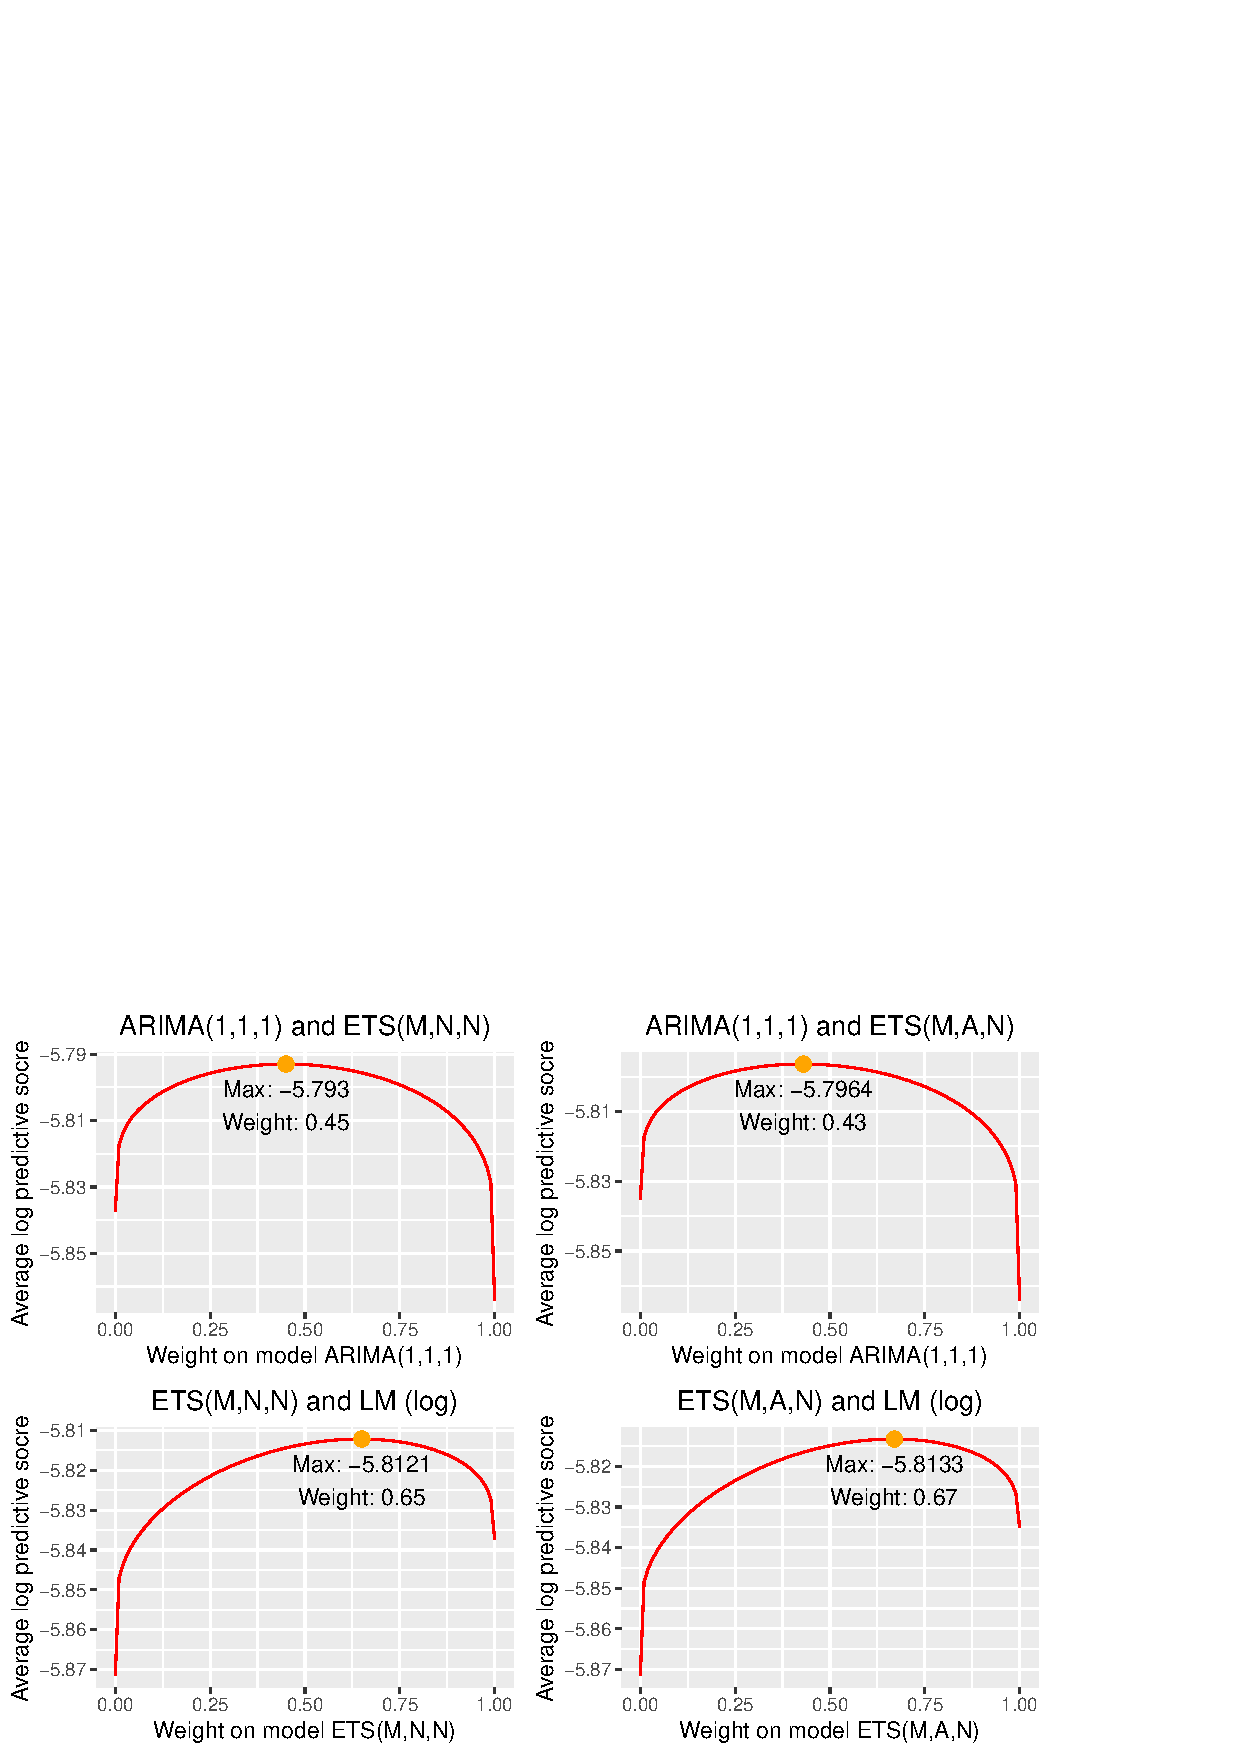
\includegraphics{figures/best4.pdf}
\begin{flushleft}
{\footnotesize The weights on the first model is in the x-axis and the corresponding average log predictive scores are on the y-axis. Constitutent models are stated in the title. The orange point represent the highest average log score of a specific combination. Its value and the corresponding optimal weight are noted below.}\\
\end{flushleft}
\label{fig:best4}
\end{figure}

\appendix

\hypertarget{appendix}{%
\chapter{Appendix}\label{appendix}}

All analyses were performed using R Statistical Software (R version 4.2.1 (2022-06-23))

Packages used are \texttt{tidyverse} \autocite{tidy19}, \texttt{dplyr} \autocite{dplyr23}, and \texttt{fpp3} \autocite{fpp23}.

\[\begin{aligned}
M_1: log(y_t) &= \phi_{0,1} + log(y_{t-1}) + \phi_{1,1}log(y)_{t-1} + \theta_{1,1}\epsilon_{t-1} + \epsilon_{t,1} \ \ \ \ \epsilon_t \stackrel{i.i.d.}{\sim} N(0,\sigma_1^2) \\
M_2: y_t &= \ell_{t-1,2}(1+\epsilon_{t,2}) \\
  \ell_{t,2} &= \ell_{t-1,2}(1+\alpha_2\epsilon_{t,2}) \\
M_3: y_t &= (\ell_{t-1}+b_{t-1}) (1+\epsilon_{t,3}) \\
  \ell_t &= \ell_{t-1}(1+\alpha\epsilon_{t,2}) \\
M_4&: y_t = \\
M_5&: y_t = 
\end{aligned}\]

\begin{equation}
  y_t - y_{t-4} = \beta (x_t-x_{t-4}) + \gamma (z_t-z_{t-4}) + \phi_1 (y_{t-1} - y_{t-5}) + \Theta_1 \varepsilon_{t-4} + \varepsilon_t
\end{equation}

\textcite{fpp3}

\printbibliography[title={Reference}]




\end{document}
